\documentclass{article}

\usepackage{microtype}

\usepackage{graphicx}
\graphicspath{{figures}}

\usepackage[backend=biber,style=ieee]{biblatex}
\addbibresource{references.bib}
\renewcommand{\bibfont}{\normalfont\small}

\usepackage{amsmath,amssymb,amsfonts,amsthm}
%\usepackage{bm}
%\usepackage{statmath}
\usepackage{upgreek}
\usepackage[retainorgcmds]{IEEEtrantools}

\newtheorem{theorem}{Theorem}
\newtheorem{corollary}{Corollary}
\newtheorem{lemma}{Lemma}
\newtheorem{proposition}{Proposition}
\newtheorem{definition}{Definition}

%\usepackage{tikz}
\usepackage{hhline}
%\usepackage{booktabs, multicol, multirow}
%\usepackage{algorthmicx}
%\usepackage{xcolor}

%\usepackage{listings}
\usepackage[cache=true]{minted}
%\usemintedstyle[python]{solarized-dark}
\setminted{obeytabs=true,tabsize=4}
\newcommand{\pyinline}[1]{\mintinline[breaklines]{python}{#1}}
%\newcommand{\pyinline}[1]{\mintinline[breaklines,breakanywhere]{python}{#1}}

\usepackage{hyperref}

\usepackage[capitalize]{cleveref}  % must be after hyperref
\crefformat{equation}{(#2#1#3)}  % used??
\crefrangeformat{equation}{(#3#1#4) to~(#5#2#6)}
\crefmultiformat{equation}{(#2#1#3)}{ and~(#2#1#3)}{, (#2#1#3)}{ and~(#2#1#3)}
\Crefname{figure}{Fig.}{Figs.}

\newlength{\eqboxstorage} \newcommand{\eqbox}[1]{ \setlength{\eqboxstorage}{\fboxsep} \setlength{\fboxsep}{6pt} \boxed{#1} \setlength{\fboxsep}{\eqboxstorage} }

\usepackage[colorinlistoftodos,color=yellow!50,linecolor=red]{todonotes}
\newcommand{\todolow}[1]{\todo[inline,color=blue!50,linecolor=red]{#1}}
\newcommand{\todolo}[1]{\todo[inline,color=green!50,linecolor=red]{#1}}
\newcommand{\todomid}[1]{\todo[inline,color=yellow!50,linecolor=red]{#1}}
\newcommand{\todohi}[1]{\todo[inline,color=orange!50,linecolor=red]{#1}}
\newcommand{\todohigh}[1]{\todo[inline,color=red!50,linecolor=red]{#1}}
\newcommand{\todocut}[1]{\todo[inline,color=violet!50,linecolor=red]{#1}}
\newcommand{\todocc}[1]{\todo[inline,color=lime!50,linecolor=red]{#1}}

\usepackage{mathfont_shortcuts}

\title{A Fascinating Paper}

\author{Paul Rademacher
    \thanks{P. Rademacher is with the Navy Center for Applied Research in Artificial Intelligence, U.S. Naval Research Laboratory, Washington, DC, USA. paul.rademacher@nrl.navy.mil}
}

\begin{document}

\maketitle

\begin{abstract}
    TODO
\end{abstract}

%\thispagestyle{fancy}
%\cfoot{\begin{small} \textbf{DISTRIBUTION STATEMENT A.} Approved for public release; distribution is unlimited. \end{small}}

\section{Introduction}
\label{sec:intro}

Cite stuff \cite{sutton_rlbook}

\begin{equation}
    \Rcal = \Erm_\xrm \Lcal(\xrm)
\end{equation}

\begin{IEEEeqnarray}{rCl}
    E & = & mc^2 \; .
    \label{eq:emc2}
\end{IEEEeqnarray}

\begin{figure}
    \centering
    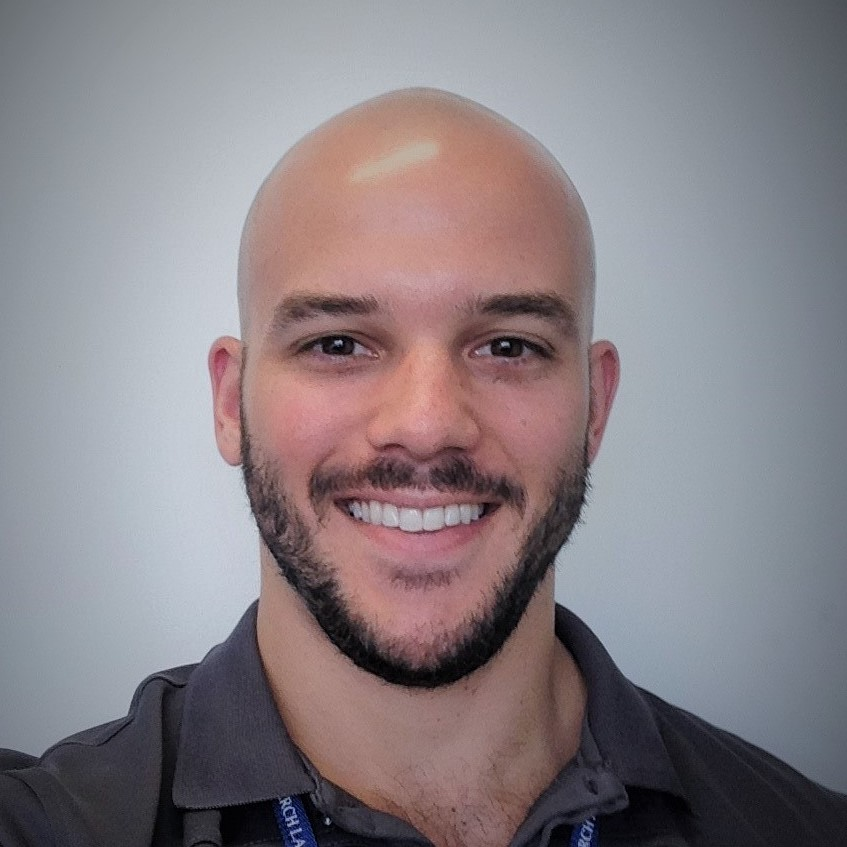
\includegraphics[width=.5\linewidth]{rademacher.jpg}
    \caption{A tremendous author}
    \label{fig:rademacher}
\end{figure}

\begin{table}[!ht]
    \centering
    \begin{tabular}{|c|c|}
        \hline
        key & val \\
        \hhline{|=|=|}
        $x$ & 0 \\ \hline
        $y$ & 1 \\ \hline
    \end{tabular}
    \caption{A table.}
    \label{tbl:table}
\end{table}

\begin{listing}
    \begin{minted}{python}
class Foo:
    def hello(self):
        print(Hello, World!)
    \end{minted}
    \caption{Listing of \pyinline{code.py}}
    \label{lst:code}
\end{listing}

\section{Conclusion}

Reference stuff, such as \cref{sec:intro}.

%\bibliographystyle{IEEEtran}
%\bibliography{../../References/PhD_refs}
\printbibliography

\appendix

\section{Stuff}
TODO

\end{document}
